\begin{graphicspathcontext}{{./chapters/sarl/imgs/},{./chapters/sarl/imgs/auto/},\old}

\begin{frame}{What Is a Behavior?}
	\begin{block}{Definition}
		A \emph{behavior} maps a collection of \emph{perceptions} (represented by \emph{events}) to a sequence of \textbf{actions}
	\end{block}
	\bigskip
	\begin{itemize}
	\item A behavior is a \emph{modular piece of agent logic}
	\item It can be \emph{dynamically added or removed} from an agent at runtime
	\item It always \emph{belongs to one agent} (its \emph{owner})
	\item It shares the \emph{skills} of its owner agent
	\end{itemize}
	\bigskip
	\begin{alertblock}{Key idea}
		Instead of writing \emph{all} agent logic in one place, split it into cohesive, reusable \emph{behaviors}
	\end{alertblock}
\end{frame}

\begin{frame}[fragile]{Declaring a Behavior}
	A behavior is introduced with the \code{behavior} keyword \\[.25cm]
	\begin{columns}
		\begin{column}[t]{.5\linewidth}
			\Emph{Minimal (empty) behavior:}
			\begin{sarllisting}
behavior MyBehavior {
}
			\end{sarllisting}
			\medskip
			\Emph{With attributes (mental state):}
			\begin{sarllisting}
behavior MyBehavior {
	var counter : int = 0
	val label : String = "ok"
}
			\end{sarllisting}
		\end{column}
		\begin{column}[t]{.5\linewidth}
			\Emph{With actions (methods):}
			\begin{sarllisting}
behavior MyBehavior {
	uses Logging
	def greet {
		info("Hello!")
	}
}
			\end{sarllisting}
		\end{column}
	\end{columns}
\end{frame}

\begin{frame}[fragile]{Reactive vs.\ Pro-active Units}
	\begin{columns}
		\begin{column}[t]{.5\linewidth}
			\Emph{Reactive} — triggered by an event
			\begin{sarllisting}
behavior MyBehavior {
	uses Logging
	// optional guard in [ ]
	on SomethingChanged
	   [occurrence.value > 0] {
		info("Value changed!")
	}
}
			\end{sarllisting}
			\vspace{-.5cm}
			\begin{itemize}
			\item \code{on EventName [guard] \{ ... \}}
			\item \code{occurrence} is the received event
			\item Guard is \emph{optional}
			\item Multiple handlers run \emph{in parallel}
			\end{itemize}
		\end{column}
		\begin{column}[t]{.5\linewidth}
			\Emph{Pro-active} — self-initiated, scheduled
			\begin{sarllisting}
behavior MyBehavior {
	uses Schedules, Logging
	on Initialize {
		every(1.seconds) [
			info("I act alone!")
		]
	}
}
			\end{sarllisting}
			\vspace{-.25cm}
			\begin{itemize}
			\item The behavior \emph{schedules itself}
			\item Uses the \code{Schedules} built-in capacity
			\item No external event needed
			\end{itemize}
		\end{column}
	\end{columns}
\end{frame}

\begin{frame}[fragile]{Lifecycle of a Behavior}
	A behavior has its own \emph{lifecycle}, mirroring the agent's:
	\begin{stabularx}{lXX}
	\tabularhead{Event}{When?}{Typical use} \\
	\code{Initialize} & Behavior registered to agent & Initialise local state \\
	\hline
	Any event & While active & React / schedule tasks \\
	\hline
	\code{Destroy} & Behavior unregistered & Release resources \\
	\end{stabularx}
	\medskip
	\begin{sarllisting}
behavior MyBehavior {
	uses Logging
	on Initialize { info("Behavior started") }
	on Destroy    { info("Behavior stopped") }
}
	\end{sarllisting}
\end{frame}

\begin{frame}[fragile]{Relation Between Agent and Behavior}
	\begin{columns}
		\begin{column}{.7\linewidth}
			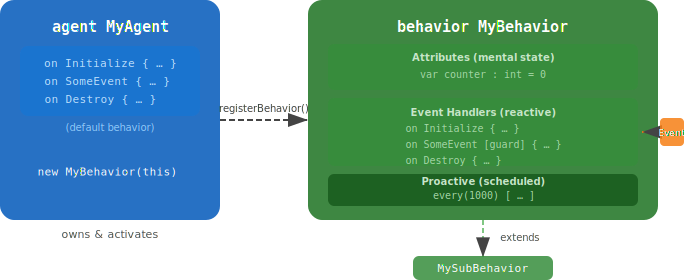
\includegraphics{sarl_behavior_agent}
		\end{column}
		\begin{column}{.3\linewidth}
			\smaller
			\Emph{How to attach a behavior to an agent:}
			\begin{sarllisting}[basicstyle=\tiny]
agent MyAgent {
	uses Behaviors

	on Initialize {
		// 1. instantiate
		var b = new MyBehavior(this)
		// 2. register
		registerBehavior(b)
	}
}
			\end{sarllisting}
			\vspace{-.5cm}
			\begin{itemize}
			\item \code{this} passes the \emph{agent as owner}
			\item \code{registerBehavior} activates event reception
			\item \code{unregisterBehavior} removes it
			\end{itemize}
		\end{column}
	\end{columns}
\end{frame}

\begin{frame}[t,fragile]{Behavior Inheritance}
	Like classes, a behavior can \emph{extend} another behavior (single inheritance):
	\begin{sarllisting}
behavior BaseBehavior {
	protected var data : String
}

behavior SpecialBehavior
         extends BaseBehavior {
	uses Logging
	on SomeEvent {
		// inherited attribute
		info("data = " + data)
	}
}
	\end{sarllisting}
	\vspace{-1cm}
	\begin{itemize}
	\item Promotes \emph{reuse} and \emph{specialisation}
	\item All \code{on Initialize} handlers from the hierarchy are run \emph{in parallel}
	\item Use \code{abstract} to create template behaviors; \code{final} to prevent further extension
	\end{itemize}
\end{frame}

\begin{frame}[fragile]{Using Capacities Inside a Behavior}
	A behavior \emph{inherits the skills} of its owner agent.
	It can also \emph{assign new skills} to the agent.
	\vspace{.25cm}
	\begin{columns}
		\begin{column}[t]{.5\linewidth}
			\Emph{Using an existing capacity:}
			\begin{sarllisting}
behavior MyBehavior {
	uses Logging, Schedules
	on SomeEvent {
		info("event received")
	}
}
			\end{sarllisting}
			\vspace{-1cm}
			\code{uses} keyword imports the capacity as an \emph{extension method}
		\end{column}
		\begin{column}[t]{.5\linewidth}
			\Emph{Assigning a skill to the agent:}
			\begin{sarllisting}
behavior MyBehavior {
	new (owner : Agent) {
		super(owner)
		setSkill(
			new MySkill(),
			typeof(MyCap))
		}
	}
			\end{sarllisting}
			\vspace{-1cm}
			Behavior can equip its agent with new capabilities at construction time
		\end{column}
	\end{columns}
\end{frame}

\end{graphicspathcontext}

\endinput

